\documentclass[11pt,a4paper,titlepage,oneside]{report}
\usepackage{titling}
\usepackage{graphicx}
\usepackage{mathtools}
\usepackage{lmodern}
\usepackage{amsmath}
\usepackage{float}
\usepackage{subfig}
\usepackage{listings}
\usepackage[hidelinks]{hyperref}

%% Memoir layout setup

%% NOTE: You are strongly advised not to change any of them unless you
%% know what you are doing.  These settings strongly interact in the
%% final look of the document.

% Dependencies
\usepackage{bfhlogo}
\usepackage{etoolbox}% http://ctan.org/pkg/etoolbox

\makeatletter
%%begin novalidate
%% Titlepage adjustments
\pretitle{\vspace{0pt plus 0.7fill}\begin{center}\Huge}
\posttitle{\end{center}\par}
\preauthor{\par\begin{center}\let\and\\\Large}
\postauthor{\end{center}}
\predate{\par\begin{center}\Large}
\postdate{\end{center}}
%%end novalidate
\def\@advisors{}
\newcommand{\advisors}[1]{\def\@advisors{#1}}
\def\@department{}
\newcommand{\department}[1]{\def\@department{#1}}
\def\@thesistype{}
\newcommand{\thesistype}[1]{\def\@thesistype{#1}}

\renewcommand{\maketitlehooka}{\noindent\bfhlogo[2cm]}

\renewcommand{\maketitlehookb}{\vspace{1in}%
  \par\begin{center}\Large\sffamily\@thesistype\end{center}}

\renewcommand{\maketitlehookd}{%
  \vfill\par
  \begin{flushright}
    \sffamily
    \@advisors\par
    \@department, BFH
  \end{flushright}
}

% Fix the chapters (unnecessary space)
\patchcmd{\@makechapterhead}{\vspace*{50\p@}}{}{}{}% Removes space above \chapter head
\patchcmd{\@makeschapterhead}{\vspace*{50\p@}}{}{}{}% Removes space above \chapter* head

\makeatother

\setlength{\droptitle}{-48pt}


\setlength{\parindent}{0pt}

\title{ORB Slam Point Cloud generation on Apalis iMX8}
\author{Stefan Eichenberger}
\date{December 2018}
\advisors{Marcus Hudritsch}
\department{TSM CPVR Lab}

\lstset{
	basicstyle=\ttfamily\tiny
}

\begin{document}
\maketitle

\begin{abstract}
	For robotic navigation a map of it's environment is required. Robots often have constraints regarding processor performance. This work analyzes different approaches in regards of their ability to run on an embedded processor using a stereo camera.
\end{abstract}

\section*{Executive Summary}
Simultaneous Location and Mapping (SLAM) is an important topic in computer vision today. The possibilities for this technology are infinite. SLAM can be used for navigation, object recognition and augmented reality. Often this algorithms need a high performance graphics card or a high performance processor. For industrial and robotics purposes space, thermal and power constraints don't allow the usage of a high performance CPUs. This work analyzes one specific SLAM algorithm on how it performs on a modern embedded ARM CPU. The final goal is to have a system available that generates a dense point cloud that can be later used to extract a map of the environment.\\\\
As embedded CPU we use an iMX8 Quad Max from NXP with hardware provided by Toradex. This processor is an early silicon and not available publicly yet. It is one of the fastest embedded processor available for industrial purposes available today.\\

\tableofcontents

\chapter{Introduction}
For robot navigation we have several possibilities today. Navigation systems can use IMUs, magneto meters, radio signals and for outdoor navigation GPS. Humans however, do a lot of navigation by eye. Today we have almost more and more computational power available and therefore computer vision becomes important. One field in computer vision is SLAM where we try to create a map of the environment and estimate the pose of the camera based on images.\\\\
In this project we analyze the performance of ORB SLAM \cite{orbslam} running on an iMX8QM. We use a Stereo Camera for creating a point cloud. By using a Stereo Camera we are able to reconstruct a point cloud with a known scale.\\\\
After porting ORB SLAM to the iMX8 we analyze the performance issues and start a discussion about possible alternatives.

\section{Apalis iMX8QM}

Toradex is interested to see some new applications and demos running on their new Apalis iMX8QM. Therefore, we concluded to try to port a computer vision application like SLAM to this platform. One area where NXP tries to place the iMX8 is computer vision in industry and automation, that's why it should be a good fit for this type of application. NXP has launched different types of iMX8. Today available is only the iMX8M which is performance wise placed between the iMX8 and the iMX8X. The Apalis iMX8QM features the most performant variant of the iMX8.

\subsection{Features}

The iMX8QM has the following features:
\begin{itemize}
  \item Two Cortex A72 high performance processors
  \item Four Cortex A53 low power processors
  \item Two Cotex M4 realtime processors 
  \item Two Vivante GC7000 GPUs for graphics and GPGPU
  \item Industrial temperature range from -40°C to 85°C
\end{itemize}

\section{Goals}
The goal of this project work are the followings:
\begin{itemize}
\item Porting ORB SLAM to Apalis iMX8
\item Analyzing different possibilities to speed up the algorithm
\item Adding an extension to create a dense cloud
\item Starting discussion about possible alternatives to ORB SLAM
\end{itemize}

\section{Time Plan}

The project was planned to end on beginning of January. The concept phase started well. Unfortunately, standard ORB SLAM doesn't perform very well in the standard implementation. First optimizations only improved the performance a little bit. However, we decided then to do a dense cloud generation first, to show a possible implementation. The time plan of this project is shown in figure \ref{fig:timeplan}.
\begin{figure}[H]
	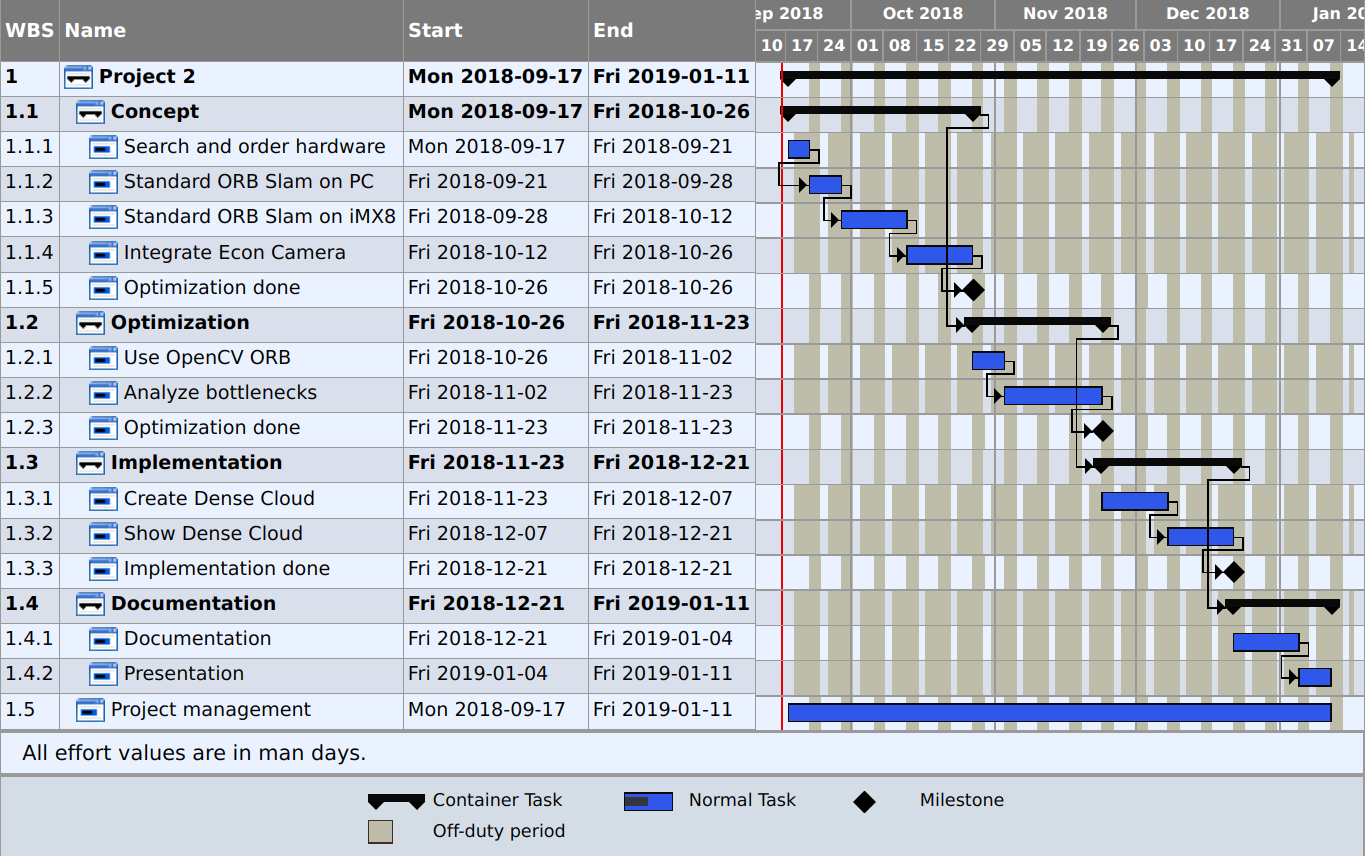
\includegraphics[width=1.0\textwidth]{img/timeplan.png}
	\caption{Time Plan}\label{fig:timeplan}
\end{figure}

\chapter{SLAM Evaluation}

As a first task we study some existing SLAM solutions. There are two groups of SLAM systems one are indirect methods and the other one are direct methods (see figure \ref{fig:slammodes}).\\\\
On indirect methods an image is analyzed and feature points are extracted. This feature points are then matched against the second stereo image and the depth of the keypoint is calculated. For the next frame again features points on the new left image are extraced and then compared with the 3d Cloud. Through matched keypoints we can then estimated the translation and rotation between the two captures.\\\\
Direct methods on the other hand operated directly on intensity variances. This means the intensities differences between two images is tried to minimize. This can be very computational intensive. Therefore, this methods often operated only on edges or even corners of the image, to reduce the computational effort. Such methods are called direct semi dense or direct sparse methods.\\\\
In the next section we will discuss the differences between monocular SLAM and stereo SLAM. We will see that they are quite similar but that stereo SLAM has some advantages over monocular SLAM.

\begin{figure}[H]
	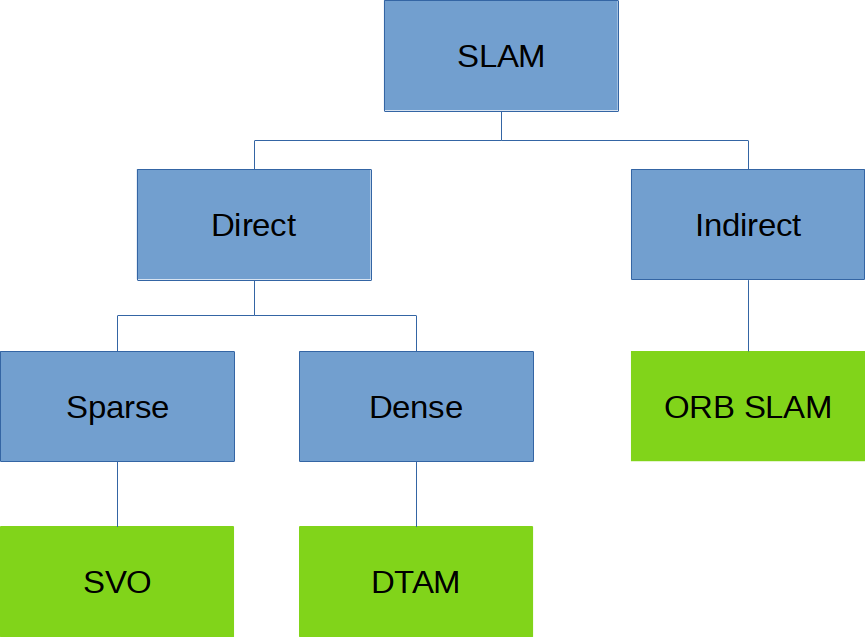
\includegraphics[width=1.0\textwidth]{img/slam_modes.png}
	\caption{SLAM Modes}\label{fig:slammodes}
\end{figure}

\section{Stereo vs Mono}

In this project the focus lays on Stereo SLAM. A lot of todays paper focus more on monocular SLAM. The reason for that is that 1. Monocular cameras are cheaper and 2. Monocular cameras are available in Smartphones. Monocular SLAM has two main problem. First an initialization process needs to estimated the movement between two frames. A 3D point cloud can only be produced with two images where the camera position was known. In the monocular the position of two images is random therefore it needs some guessing and optimization to find the pose and transformation until a first point cloud can be generated. Event if the initialization succeeded we don't know the moving distance in the real world between the two images. This means we have to guess some scale factor which will be unknown for the whole tracking. This means monocular SLAM finds out movement distances between two poses with regards to it's initialization moving distance but without a known scale. In modern Smartphones this is fixed by using IMU data which gives you the real world movement and therefore the scale factor.\\
For stereo SLAM we don't have this issues. For each camera pose we get two images with known the distance between the two camera sensors (baseline). Therefore, we can theoretically calculate the depth of each pixel in real world distance. From this we can already generate a point cloud assuming that the initial camera pose starts at (0,0,0) world coordinate. We therefore have an instantaneous initialization and can calculate the real world position in e.g. meters.\\
Tracking between two camera poses is however similar for monocular and stereo SLAM. For stereo SLAM it is often only done on the left image. However keypoints can again be inserted immediately on stereo cameras without the need of using a second camera pose. This cam make stereo SLAM more robust against loose of tracking.\\
In the next section we will compare indirect SLAM methods against direct SLAM methods.

\section{Indirect method}

A well documented indirect method is ORB SLAM \cite{orbslam}. Stereo ORB SLAM extracts keypoints on the left and right image. It matches the keypoints on the left and right image and calculates the depth of each point. Based on this points it generates a first point cloud. For the next camera pose it extracts again the keypoints. This keypoints are then matched against the keypoints in the 3d cloud and the translation and rotations between the two poses is calculated.\\\\
Because we know the descriptor of each keypoint we can use triangulation and RANSAC to estimate the pose.\\\\
Indirect methods have the advantage that the pose estimation can be done direct and isn't computational expensive. On the other side the computation of keypoint features is more expensive.

\section{Direct method}

There are two different kinds of direct methods. Dense direct methods and sparse direct methods. The difference is that for Dense direct methods all pixels of the image are used to do the tracking while for sparse methods only a subset of pixels of the image is used.

\subsection{Dense}

There are not that many dense SLAMs. One is DTAM which uses the intensity values of the whole image to do the pose estimation. The idea is to minimize the energy between two images by optimizing the camera pose. The energy defined at a specific position in the image is defined as shown in \ref{eq:pixel_energy}. To estimate the Pose it tries to find a P that minimizes $E_{t}$ as shown in \ref{eq:total_energy}.
\begin{equation}\label{eq:pixel_energy}
  E_{u}=I_1(u)-I_2(P*U)
\end{equation}
Where:
\begin{align*}
  E_{u}		&: \text{Energy at a specific position}\\
  I_{1/2}:	&: \text{Image 1/2}\\
  u:		&: \text{Position in image} \\
  P:		&: \text{Pose of the camera} \\
  U:		&: \text{Position of x in 3D}
\end{align*}
\begin{equation}\label{eq:total_energy}
  E_{t}=\min(\sum_{x=0}^X\sum_{y=0}^YE_u)
\end{equation}

One of the biggest advantages of using a direct dense method is that we receive a dense point cloud which can be used directly to create maps and 3d objects. A big disadvantage is however that they are quite computational expensive. Therefore they are unfortunately not appropriate for embedded devices.

\subsection{Sparse}

% TODO: Add references to DSO, FAST and LSD
Sparse direct SLAMs like SVO don't optimize the Energy over the whole image but use some sparse points instead. One possibility of a sparse point is e.g. a corner point found by FAST. Similar to sparse methods there are semi dense methods which try to minimize the energy with several points laying on edges. They can e.g. be found by Canny Edge detection or DoG. The advantage of sparse and semi dense are that such methods are less computational expensive than dense methods.\\\\

Sparse direct methods don't create dense clouds immediately however they are able to work on weaker keypoints than indirect methods. Therefore they can create denser clouds than e.g. ORB SLAM. They can also be computational less expensive than indirect methods because they don't have to calculate expensive features.

\section{Decision}

We decided to give ORB SLAM a first try because of the open source availability of this algorithm. Also there is some experience at the CPVR lab with this algorithm and 8-12 fps were achieved on a modern smartphone. The iMX8 has a processor with similar power as todays mid end smartphone therefor the hope is to achieve similar performances.

\chapter{Camera Evaluation}

To do stereo vision we of course need a stereo camera. There are a few stereo camera available on the market and it would also be possible to build a stereo camera on our own.

\section{ZED}
The ZED camera is an extremely promising camera for stereo vision. Here a list of the features:
\begin{itemize}
	\item Full HD color images with 30fps
	\item USB3.0
	\item UVC compliant
	\item Linux SDK
	\item Baseline 120mm
	\item IMU sensor with 6DoF
	\item Price: 449\$
\end{itemize}

To run their SDK a Dual Core CPU with 2.3 GHz and CUDA > 3.0 is required. However, it's also possible to use the camera without their SDK.

\section{ECON Tara}
The ECON Tara is another stereo camera. In comparison to the ZED camera it delivers reduced resolution and only gray scale images.
\begin{itemize}
	\item 752x480 gray scale images with 60fps
	\item USB3.0
	\item Global Shutter Camera
	\item UVC compliant
	\item Baseline 60mm
	\item IMU sensor with 6DoF
	\item Open Source SDK
	\item Price: 149\$
\end{itemize}

\section{Intel RealSense D430}
The Intel RealSense camera is a infrared stereo camera. In comparison to RGB stereo camera it uses infrared images for stereo vision. Additionally it also has an RGB sensor.
\begin{itemize}
	\item 1280x720 with 90fps (IR), 1920x1080 with 30fps (RGB)
	\item USB3.0
	\item Global Shutter Camera
	\item UVC compilant (kernel patch required)
	\item Baseline 50mm
	\item Open Source SDK (librealsense)
	\item Price: 179\$
\end{itemize}

\section{Decision}

Because of the good price ration and because it is a conventional stereo camera, we decide to use the ECON Tara stereo camera. However, the Intel RealSense camera would be a great fit as well because it delivers a depth image directly. This would reduce the CPU load because the camera does the depth calculation. If Full HD is required the ZED would be the perfect fit, however keep in mind that for embedded systems Full HD processing may not be possible.

\chapter{Camera Calibration}

Camera calibration is necessary to find a model that expresses the properties of a camera. Properties of a camera are:

\begin{itemize}
	\item Focal length of the camera lense
	\item Principal point on the camera sensor, where the z axis of the cameras coordinate system goes through.
	\item Distortion of the camera lense
	\item Size of a pixel
\end{itemize}

If we once know the camera model and the camera position, we can project virtual objects into a real world image. Figure \ref{fig:model} shows an image of a checkerboard where we project a virtual cube onto. One camera model in this image took distortion into account while the other one ignored it.
\begin{figure}[H]
  \begin{center}
		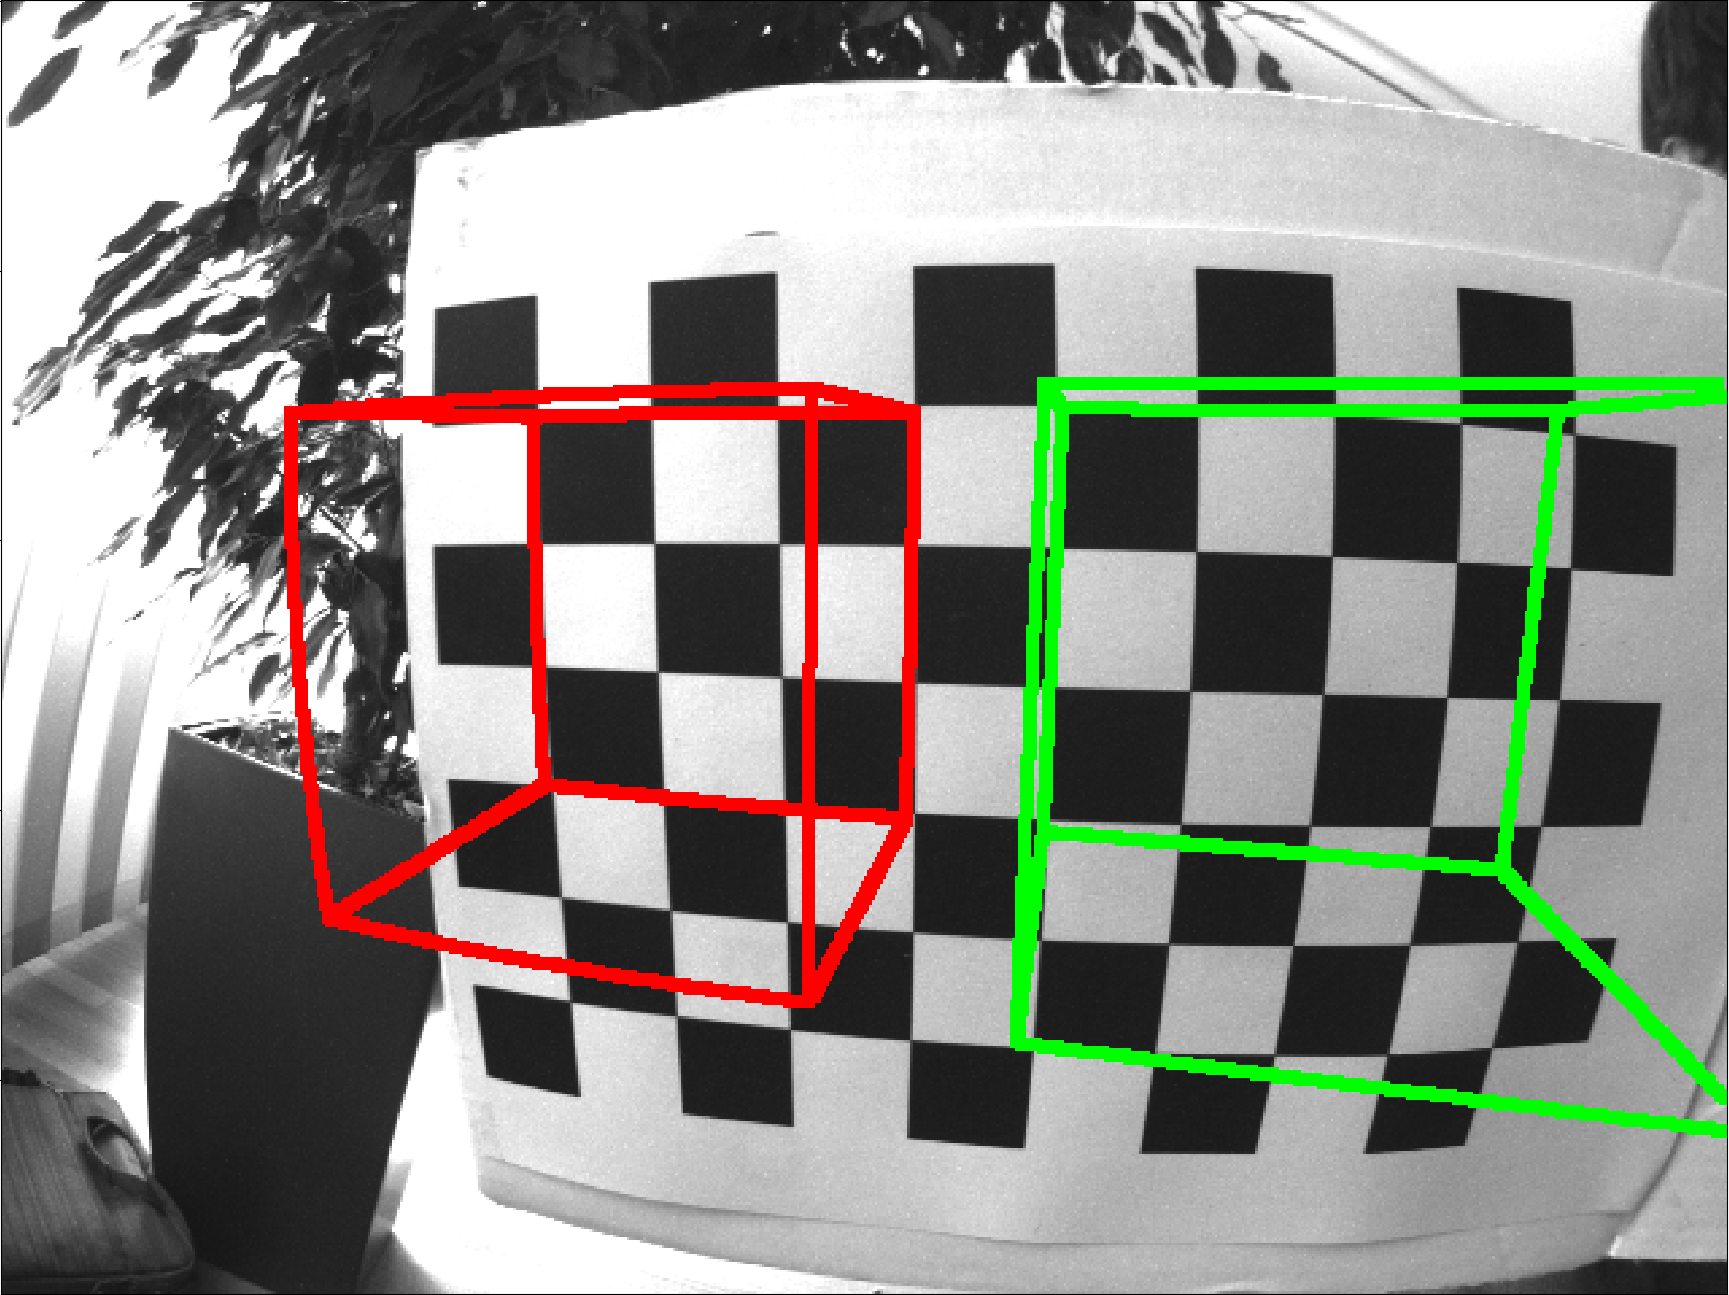
\includegraphics[width=1.0\textwidth]{img/model.png}
  \end{center}
	\caption{Applied camera model with (red) and without(green) distortion}\label{fig:model}
\end{figure}

Additional to the above parameters we need to align the images of the left and right camera in stereo vision. This process is called rectifying. The cameras aren't perfectly aligned in horizontal direction however we need to have them aligned because this makes it possible to search for correspondence only on the epipolar line. Further the cameras are slightly rotated which means we must inverse rotate the image to have a perfect alignment. So additional to the properties of the camera we need to know the following parameters:
\begin{itemize}
	\item Rotation matrix of the right camera in regards to the left
	\item Y offset of the right and left camera in pixels
	\item Maximum overlapping region of left and right camera
\end{itemize}


\section{Camera Model}

The camera model expresses how any point in the three-dimensional space is projected onto a two-dimensional image. As a first approximation it assumes that all rays are going trough one point. This is called the pinhole camera model \ref{fig:projection}a. Given this assumption we can describe the projection of a 3D point onto a 2D image as shown in equation \ref{eq:cm}. We calculate the pixel location $x,y$ on the image by normalizing with $s$ as show in equation \ref{eq:cm_normalized} \cite{rvc}.
\begin{equation}\label{eq:cm}
  \begin{pmatrix}
		f_x & \gamma & c_x \\
		0 & f_y & c_y \\
		0 & 0 & 1 \\
	\end{pmatrix}*
	\begin{pmatrix}
		r_{00} & r_{01} & r_{02} & t_x \\
		r_{10} & r_{11} & r_{12} & t_y \\
		r_{20} & r_{21} & r_{22} & t_z \\
	\end{pmatrix}
	\begin{pmatrix}
		X \\
		Y \\
		Z \\
		1
	\end{pmatrix}=
	\begin{pmatrix}
		u \\
		v \\
		s
  \end{pmatrix}
\end{equation}
\begin{equation}\label{eq:cm_normalized}
	\begin{pmatrix}
		x \\
		y
	\end{pmatrix}=
	\begin{pmatrix}
		u/s \\
		v/s 
  \end{pmatrix}
\end{equation}

Where:
\begin{align*}
  X,Y,Z			&: \text{point in the 3D world}\\
	u,v,s	   	&: \text{point in 2D image not normalize}\\
	x,y				&: \text{point in 2D image normalized with s}\\
	f_x,f_y  	&: \text{focal length of the camera}\\
  c_x,c_y  	&: \text{principal point}\\
  t_x,t_y,t_z	&: \text{location of the camera}\\
  r_{ij}	&: \text{part of the rotation matrix}
\end{align*}

We can describe the intuition as follows. A Point (X,Y,Z) is projected onto an image sensor (u/s,v/s) by the multiplication of the intrinsic times the extrinsic matrix. The extrinsic matrix describes where the pinhole of the camera is located in the three dimensional space. The intrinsic camera matrix describes how the camera is constructed. For example, in figure \ref{fig:projection}b we translate and rotate a point $p_i$ with the extrinsic matrix so we can describe its coordinates with the pinhole as origin. Further we transform the point with the intrinsic camera matrix onto the image sensor.\\
\em
Note:\\
In the previous section we said we also need to know the pixel size. This is true but will not appear directly in the camera model. The parameters fx and fy who are sizes in meters are expressed in pixels. They therefore include the information about pixel size.
\normalfont

\begin{figure}[H]
	\centering
	\subfloat[Pinhole model]{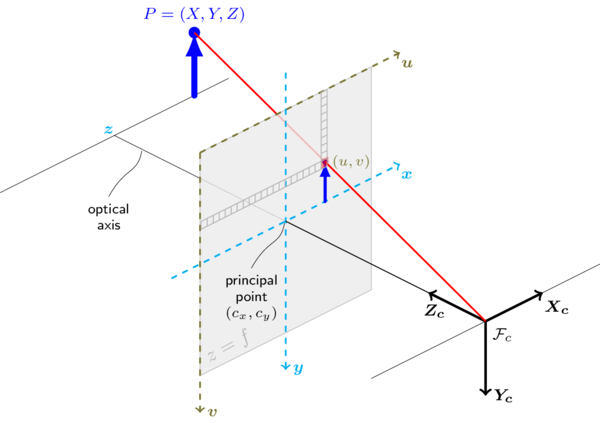
\includegraphics[width=0.5\textwidth]{img/pinhole_camera_model.png}}
	\subfloat[3D point to 2D point]{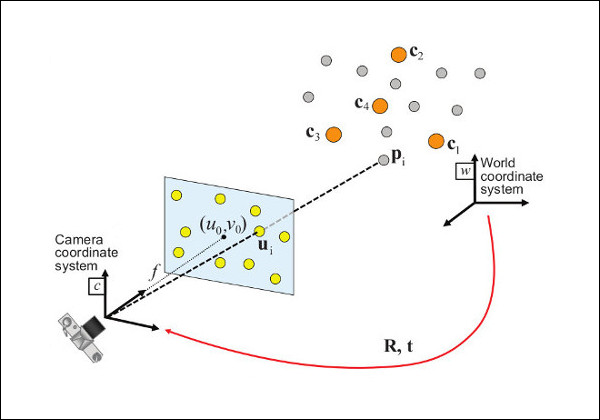
\includegraphics[width=0.5\textwidth]{img/pnp.jpg}}
	\caption{Image projection}\label{fig:projection}
\end{figure}

\section{Stereo Camera Model}

Additional to the monocular parameters we need to find out the parameters of the stereo camera. An image taken by a stereo camera normally is misaligned as shown in the top row of figure \ref{fig:stereo_calib}. The goal is to find the rotation matrix as well as the Y offset and the non overlapping part of the image (black part in figure \ref{fig:stereo_calib}).\\
While for monocular calibration a mid size checkerboard works fine a huge size of the checkerboard is much more important when doing stereo calibration. If the checkerboard is small a pixel has a much bigger effect on the final calibration data than if the checkerboard is big.

%TODO: Add proof if we have time

\begin{figure}[H]
  \begin{center}
		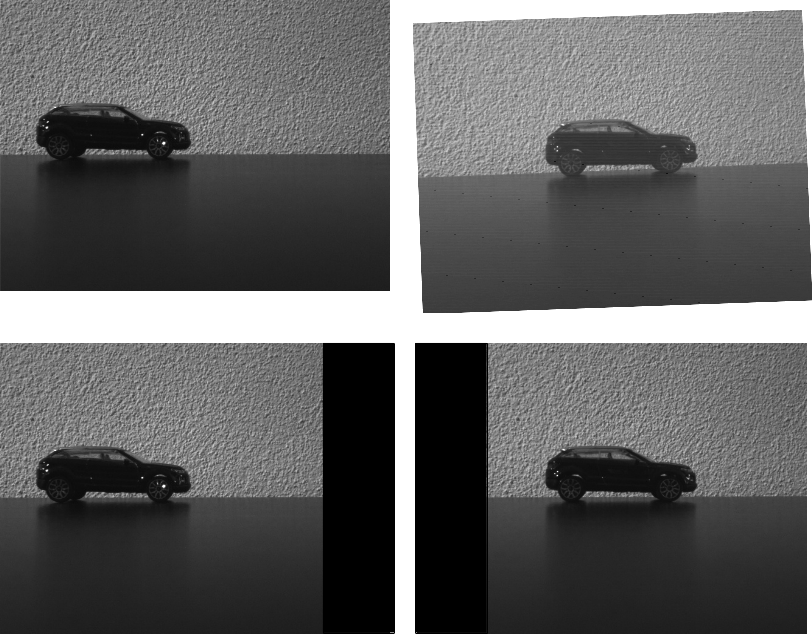
\includegraphics[width=0.9\textwidth]{img/stereo_calib.png}
  \end{center}
	\caption{Stereo Calibration, top row misaligned image, bottom row rectified images}\label{fig:stereo_calib}
\end{figure}

\chapter{ORB SLAM}\label{chap:implementation}

In this chapter we discuss more deeply how ORB SLAM works and how we port it to the iMX8 processor.

\section{How it works}
ORB SLAM tries to find corners with the FAST corner detection. This gives us points which should lay on the intersection between two edges. We call this points keypoints. At the corners we later calculate the ORB descriptors which describes the keypoint.\\
If we have a stereo image we can search for the keypoints on both images and from that calculate the depth of each point. For this we need to do the steps shown in figure \ref{fig:orb_slam2}.

\begin{figure}[H]
  \begin{center}
		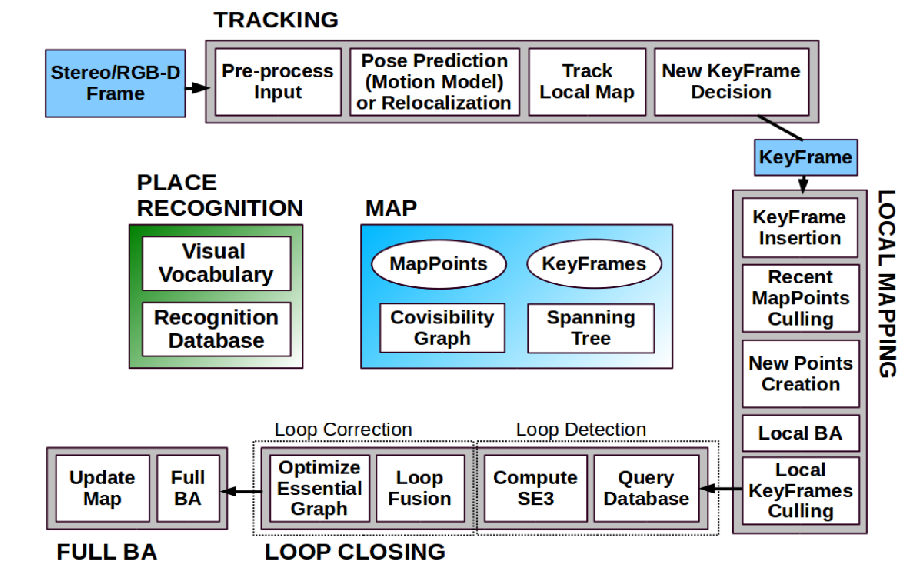
\includegraphics[width=0.9\textwidth]{img/orb_slam2.png}
  \end{center}
	\caption{ORB SLAM2 \cite{orbslam2}}\label{fig:orb_slam2}
\end{figure}

ORB SLAM uses multiple threads to improve the performance of the algorithm. \\
Tracking:
\begin{enumerate}
	\item Match descriptors from the left and the right image
	\item Calculate the difference in pixels between the keypoint on the left and on the right image
	\item Calculate the depth of the keypoint with formula shown in equation \ref{eq:depth}
	\item With known depth calculate the point position with camera as reference
	\item Match point descriptors with point descriptors from keyframe
	\item Estimate new camera pose with triangulation and RANSAC
	\item Check if this frame is a potential keyframe.
\end{enumerate}
The potential keyframe check is done by checking how many frames were captured since the last keyframe, if a lot of outliers were detected and if more than 35\% of points are new with regards to the reference keyframe.\\

Local Mapping:
\begin{enumerate}
	\item Transform the new keypoints to the global coordinate system based on the camera pose
	\item Do a bundle adjustment. It is likely that points we already know do not 100\% match the position where we see the points. Bundle adjustment fuses the position of points seen more than once.
	\item Check if more than 10\% of the points in the current frame compared to the points in all keyframes are new. If not we drop the keyframe for future use.
	\item 
\end{enumerate}

Loop Closing:
\begin{enumerate}
	\item Match latest keyframe with all keyframes stored in the database with DBoW2 \cite{dbow}
	\item Optimize correspondent point by doing bundle adjustment over key frame poses and point location
\end{enumerate}

\begin{equation}\label{eq:depth}
	d=\frac{b}{\Delta}\\
	\Delta=u_{left}-u_{right}
\end{equation}
\begin{align*}
	d &:					\text{depth}\\
	b &:					\text{baseline (distance between left and right camera)}\\
	\Delta &:			\text{Difference between x position on left and rigth image}\\
	\u_{left} &:	\text{X Position of keypoint on left image}\\
	\u_{right} &: \text{X Position of keypoint on right image}
\end{align*}

\begin{equation}\label{eq:orb_pos}
	y=\frac{d*u}{f_u}\\
	x=\frac{d*v}{f_v}
\end{equation}
\begin{align*}
	y &:				\text{Y position with camera 0}\\
	x &: 				\text{X position with camera 0}\\
	d &: 				\text{Depth=Z position with camera 0}\\
	u,v &:			\text{X,Y position on image}\\
	f_u,f_v &:	\text{Focal length}
\end{align*}

\section{Comparison Mono to Stereo}

In this work we only talk about stereo SLAM. But what are the differences to a monocular SLAM system?\\
A monocular camera can't see depth. This means that from one single image we can't estimate the keypoints in the 3D world. This means we need some kind of initialization process that will try to estimate the depth over several images. There are different strategies for solving the initialization problem. ORB SLAM calculates two models in parallel one if most points are laying on a plane and one model if most points are random distributed. In one model the Essential Matrix (Fundamental Matrix with only 5DoF) is searched while in the other model the homography matrix is searched. If the initialization succeeds one of this matrices will converge to a small reprojection error while the other wont. The new camera pose can be estimated by decomposing the converged matrix. Other approaches use a EKF and try to optimize the camera pose over the first n frames. The EKF starts with random depth values and converges after several frames to the ``real'' depth values.  For a monocular camera it is not possible to find all 6 DoF because the fundamental and homography matrix only have 5DoF. They therefore set the 6 parameter to 1 which means we don't get a real ``scale'' value. All measurements with only monocular cameras are therefore scales.

\section{Port to iMX8}\label{sec:orbport}

The iMX8 BSP is built with Yocto. NXP and Toradex provide a BSP layer which contains a kernel and all necessary proprietary libraries for OpenGL. OpenCV is already part of the image fsl-image-qt5. How we build the BSP and the SDK is out of scope of this project. Please check the following references:\\
\begin{itemize}
	\item Yocto project \cite{yocto}
	\item Toradex BSP \cite{toradex_bsp}
\end{itemize}

From the Yocto build we can also receive an SDK which contains a ARM64 toolchain that can be used to compile additional programs and libraries. This toolchain was used to build the ORB SLAM2 for the iMX8. For the following section we assume that the toolchain is installed under/opt/fsl-imx-x11/4.9.51-mx8-beta

\subsection{Pangolin}
Pangolin \cite{pangolin} is required by ORB SLAM for showing the sparse map and the camera pose. A simple git checkout of the pangolin sources is enough to receive the sources. Before building the project with CMake the following patch should be applied:
\begin{lstlisting}
diff --git a/CMakeLists.txt b/CMakeLists.txt
index 32a2d78..683ef38 100644
--- a/CMakeLists.txt
+++ b/CMakeLists.txt
@@ -15,6 +15,9 @@ SET(CPACK_DEBIAN_PACKAGE_MAINTAINER "Steven Lovegrove")
 SET(CPACK_PACKAGE_VERSION_MAJOR ${PANGOLIN_VERSION_MAJOR})
 SET(CPACK_PACKAGE_VERSION_MINOR ${PANGOLIN_VERSION_MINOR})
 SET(CPACK_PACKAGE_VERSION_PATCH "0")
+SET(CMAKE_INCLUDE_SYSTEM_FLAG_CXX "-I")
+SET(CMAKE_INCLUDE_SYSTEM_FLAG_C "-I")
+
 include(CPack)
 
 option( BUILD_EXAMPLES "Build Examples" ON )
\end{lstlisting}

After that the following commands should be done:
\begin{lstlisting}[language=bash]
. /opt/fsl-imx-x11/4.9.51-mx8-beta/environment-setup-aarch64-poky-linux
mkdir build
cd build
cmake -DCMAKE_INSTALL_PREFIX=<INSTALL_DIR> ..
make -j
make install
\end{lstlisting}

This will build the Pangolin library for ARM64. INSTALL\_DIR should point to a directory which can be used as local ``root filesystem''. This root filesystem can later be copied via scp to the iMX8.

\subsection{ORB SLAM2}
We use the sources of ORB SLAM 2 \cite{orbslam2_impl}. Instead of using the sources from ORB SLAM directly the modified sources \cite{orbslam2_se} under branch iMX8 should be used. It contains some fixes for newer compiler versions as well as additional sources for the ECON Tara camera. After checking out the sources the following commands should build the binaries:\\
\begin{lstlisting}[language=bash]
. /opt/fsl-imx-x11/4.9.51-mx8-beta/environment-setup-aarch64-poky-linux
mkdir build
cd build
cmake -DPangolin_DIR=<INSTALL_DIR/usr/lib/cmake/Pangolin> -DCMAKE_INSTALL_PREFIX=<INSTALL_DIR> ..
make -j
make install
\end{lstlisting}

This will build ORB SLAM for ARM64. INSTALL\_DIR is the same directory as it was for Pangolin. After that we can copy the whole INSTALL\_DIR to the iMX8 root directory and start econ\_stereo for starting the SLAM system.

\chapter{Densification}

ORB SLAM only delivers a very sparse map. Therefore, it can't be used e.g. for creating a map or to reconstruct 3D objects. It's focus lays on delivering a stable pose of camera rather than on creating a useful map of it's environment. In this section we discuss how we can improve ORB SLAM by densifing the point cloud. We also show a ruff implementation which however isn't state of the art as we will see later.\\
In the first section we will see how the stereo images can be used to create a depth map. The next section describes how to use the depth map to generate a point cloud. The two last sections discusses two possibilities how a depth map of several poses could be fused together. However, as we will see the current approach doesn't work as expected because the point cloud increases too fast and the algorithms slows down massively.

\section{Depth Map}

A depth map is an image that contains depth values instead of color intensities. They are normally generated from stereo cameras or from ToF cameras. We will only talk about how depth images are generated from stereo cameras. Image \ref{fig:depth} shows such an image that was generated from the images of a stereo camera.

\begin{figure}[H]
	\centering
	\subfloat[left image]{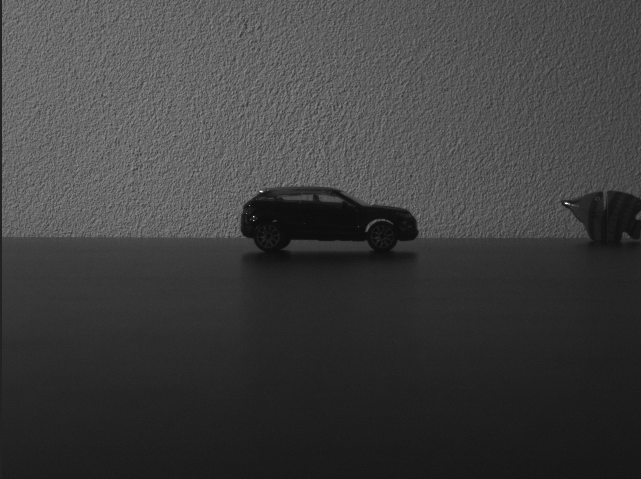
\includegraphics[height=100px]{img/disparity_left.png}}
	\subfloat[right image]{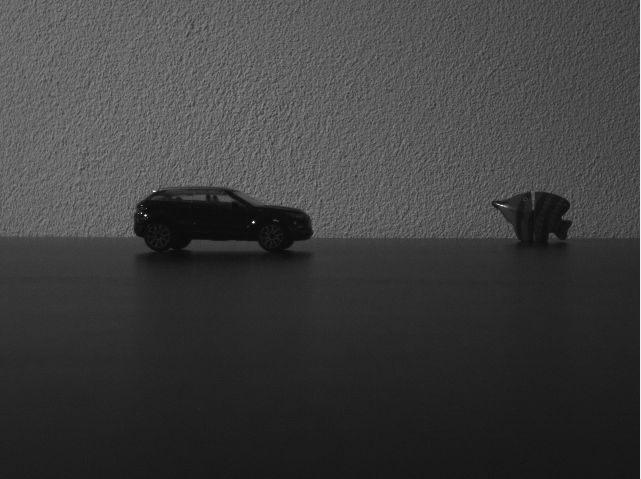
\includegraphics[height=100px]{img/disparity_right.png}}
	\subfloat[depth image]{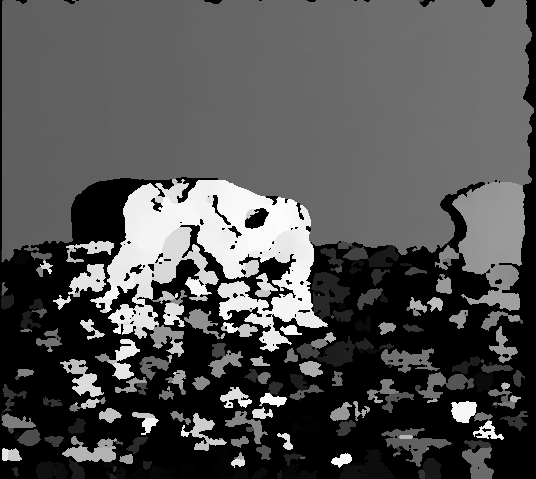
\includegraphics[height=100px]{img/disparity.png}}
	\caption{Depth image from stereo}\label{fig:depth}
\end{figure}

As we can see in figure \ref{fig:depth} the depth image is noisy in areas where the we have low or no texture. This is due to how the algorithm works. The algorithm does an intensity block matching. Because the camera is aligned horizontally the algorithm begins matching at the pixel position of the left image and matches from there to the right as shown in figure \ref{fig:disparity}. The horizontal line is also called epipolar line. The distance of a point on the left image to the right image is called disparity. An object which is farer away will have less disparity than an object which is near. A point at infinity will have a disparity of zero.

\begin{figure}[H]
  \begin{center}
		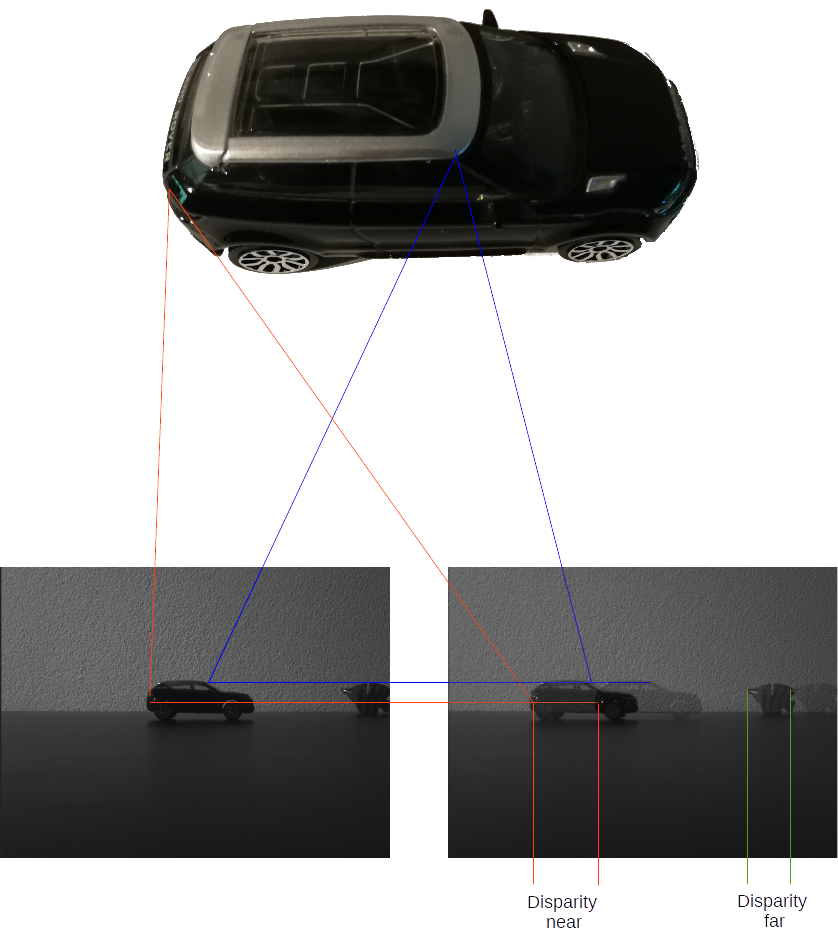
\includegraphics[width=0.9\textwidth]{img/disparity_concept.png}
  \end{center}
	\caption{Disparity with epipolar (horizontal) line, left: left image, right: right image with transparent left image}\label{fig:disparity}
\end{figure}

We use a Block Matching algorithm which matches for each pixel a template from the left image with the right image. The pixel with the lowest value is taken as best match and the offset is the disparity. However this algorithm is prone to noise therefore a modified version of this algorithm is used called Semi Global Block Matching (SGBM) \cite{sgbm}. In comparison to normal Block Matching this algorithm penalties if neighbour pixels have a big disparity difference. We additionally calculate the disparity for the left and right image so that we also get values for pixels that are only visible in one image. Further we can generate a confidence map if pixels have different disparities when we do left and right matching.

\section{Point Cloud from Depth}

From the Depth map generated by the previous section we can then calculate a dense point cloud based on the current pose. We transform the depth information into the three dimensional space. An example of such a point cloud can be seen in figure \ref{fig:pointcloud}. The point cloud is generated from the depth image by transforming each pixel with the current camera pose.

\begin{equation}\label{eq:point_cloud_depth}
	\begin{pmatrix}
			X \\
			Y \\
			Z
	\end{pmatrix}=
	\begin{pmatrix}
		r_{00} & r_{01} & r_{02} & t_x \\
		r_{10} & r_{11} & r_{12} & t_y \\
		r_{20} & r_{21} & r_{22} & t_z \\
	\end{pmatrix}*
	\begin{pmatrix}
		x,
		y,
		d,
		1
	\end{pmatrix}
\end{equation}
\begin{align*}
	X,Y,Z &:			\text{World position of the pixel}\\
	r_{ij} &:			\text{Rotation elements of pose}\\
	t_{x,y,z} &:	\text{Translation elements of pose}\\
	x,y:					\text{u,v translated to world, see \ref{eq:orb_pos}}\\
	d &:					\text{depth}
\end{align*}

\begin{figure}[H]
  \begin{center}
		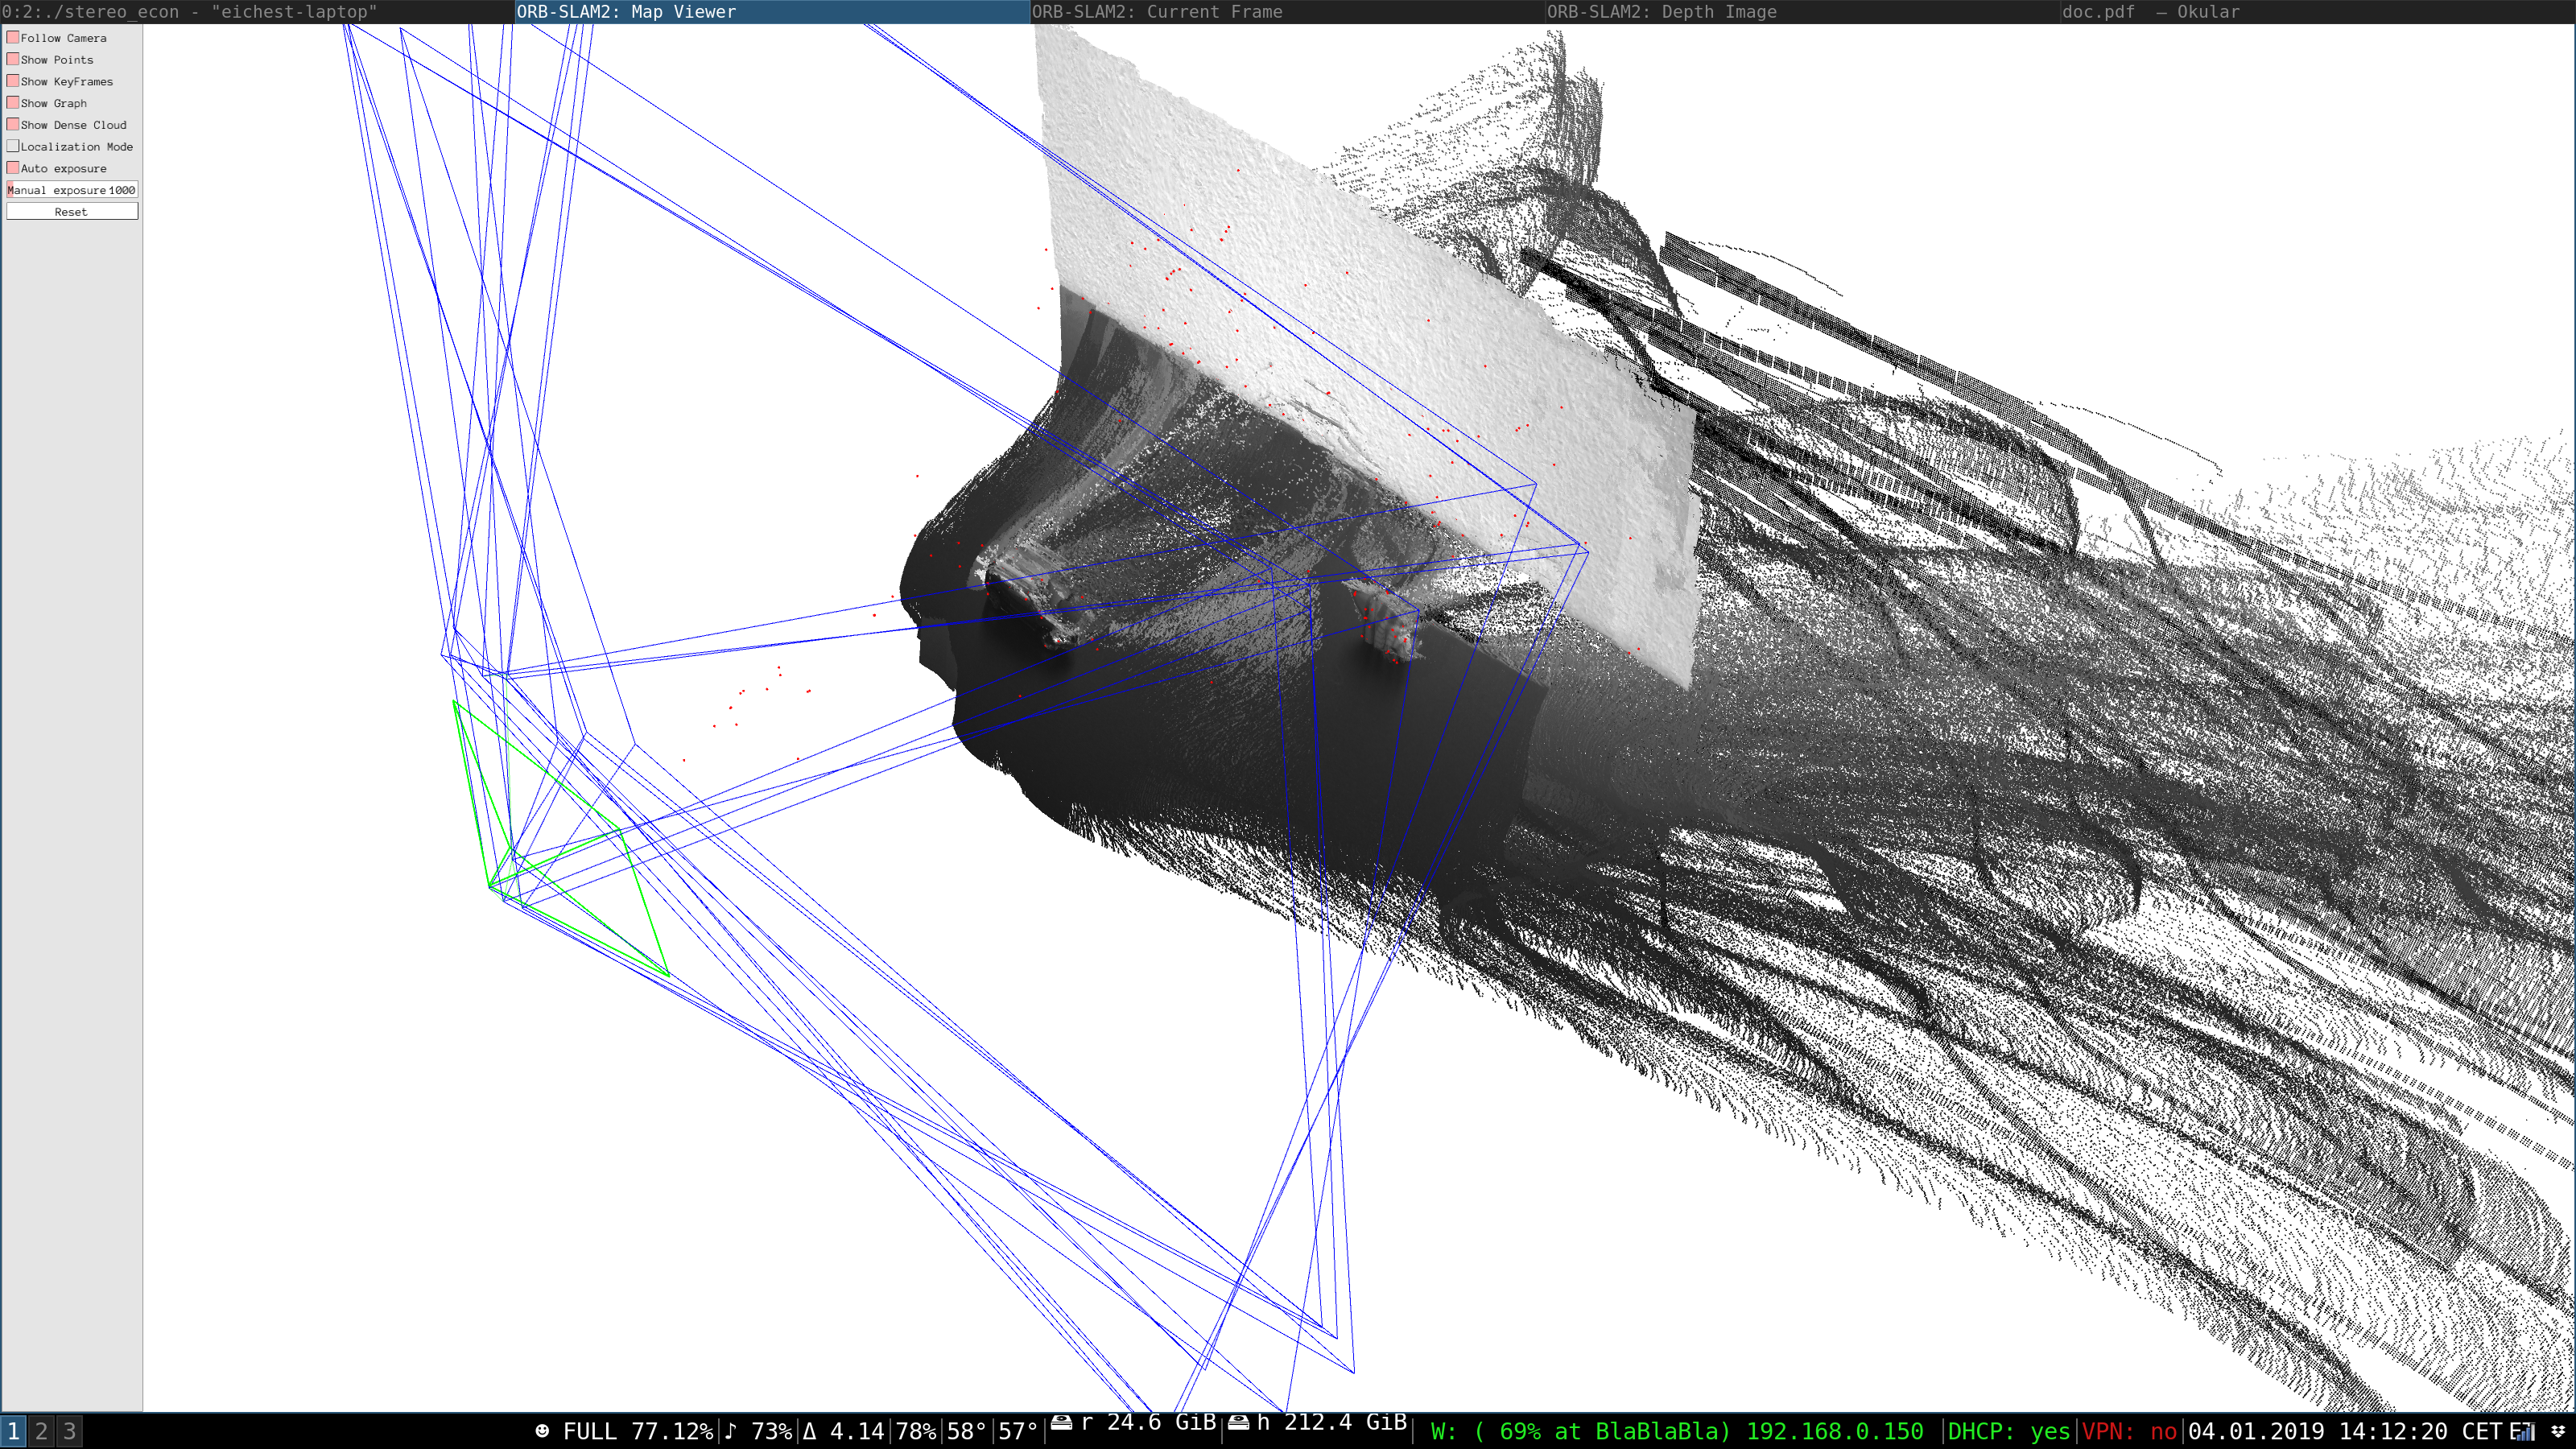
\includegraphics[width=0.9\textwidth]{img/pointcloud.png}
  \end{center}
	\caption{Dense point cloud generated different key frames}\label{fig:pointcloud}
\end{figure}

To reduce the CPU load we only add new dense points to the cloud for keyframes. What we can see in figure \ref{fig:pointcloud} is that because of the uncertainty of the depth map we have tons of outliers. Further we don't fuse points at the same location therefore we generate a lot of points that have the same position within a statistic probability.

\section{Point Cloud fusion}

There are different papers that describe the problem of point cloud fusion. If you have two views that partially show the same region you will always have to merge the overlapping part. Here I would like to shortly point out two possibilities for that. REMODE and Volumetric 3D Mapping.

\subsection{REMODE}

REMODE uses a probabilistic approach to fuse data from different views. Only points that have a high enough probability for being there are actually drawn on the 3D map. This generates a semi dens point cloud which has a high probability of being true. However it requires a lot of frames seeing the same scene for getting high accuracy, this is exactly what we try to avoid because we already have problems to perform well with our current approach. Therefore this algorithm can't be used in embedded systems for our dense cloud.

\subsection{Volumetric 3D Mapping}

The approach of using a volumetric 3D mapping is quite interesting. The algorithm is designed to run on a CPU only. It assigns a box to each 3D pixel and grids this boxes in an octree. If a new pixel should entered the algorithm check whether it would fix in an existing box. Unfortunately, a short test implementation showed that also this approach would use too much CPU power. Therefore, we have to think about a different approach.

\chapter{Reflection}

In this chapter we reflect over the current status of this work. We analyse the achievements and see if we can improve the approach to achieve realtime location and mapping.

\section{Results}

The current implementation is heavily based on the original ORB SLAM2 implementation as described in section \ref{sec:orbport}. Because we used normal ORB SLAM the results from the original paper are still valid. However, what we are interested in is the realtime frame rate and the therefore the time used per frame. The original ORB SLAM2 implementation calculates exactly this time per frame and writes out the mean and median time after each run. For comparison we used the KITTI04 dataset with 271 images. The resolution of each image is 1226x370 where the ECON Tara has a resolution of 752x480. The KITTI dataset is a standard benchmark for SLAM therefore this one was taken. In comparison to Euroc another dataset it has smaller sequences and finishes therefore faster.\\\

We compare the ORB SLAM ORB implementation with the ORB implementation from OpenCV. To be fair we reduce the feature count from 1000 to 800 because OpenCV ORB normally finds more features than the ORB SLAM implementation. The bigger the point cloud gets the slower the algorithm performs, therefore it wouldn't be a fair comparison.

median tracking time: 0.358698
mean tracking time: 0.362126


\begin{table}
	\begin{tabular}{  | l | l | l | l | l | l | }
		\hline
		\textbf{CPU} & \textbf{Impl.} & \textbf{feat.} & \textbf{feat. det.} & \textbf{median tt} & \textbf{mean tt} \\ \hline
		iMX8 & ORB & 1000 &  548 & 0.18307 & 0.185202 \\ \hline
		iMX8 & ORB, Linux scheduled & 1000 & 548 & 0.390867 & 0.387753 \\ \hline
		iMX8 & OpenCV & 1000 & 757 & 0.190571 & 0.210072 \\ \hline
		iMX8 & OpenCV & 800 & 610 & \textbf{0.155441} & \textbf{0.167176} \\ \hline
		iMX8 & OpenCV, Linux scheduled & 800 & 610 & 0.358689 & 0.362126 \\ \hline
		iMX8 & OpenCV OpenCL & 800 & 610 & 0.50622 & 0.771859 \\ \hline
		i5-7Y54 & ORB & 1000 & 546 & 0.18884 & 0.184628 \\ \hline
		i5-7Y54 & OpenCV & 1000 & 756 & 0.154901 & 0.152786 \\ \hline
		i5-7Y54 & OpenCV & 800 & 610 & 0.135715 & 0.132304 \\ \hline
	\end{tabular}
	\caption{Comparison of ORB SLAM tracking time in KITTI04 using ORB or OpenCV implementation}
  \label{tab:result}
\end{table}

As we can see from table \ref{tab:result} we can achieve the best timings on the iMX8 when using the OpenCV ORB SLAM implementation. We could extend this version so that it behaves the same as the ORB SLAM implementation and would still benefit from the improvement. However, we are still at a very low frame rate of around 6 frames per seconds. When we compare this result to a i5-7Y54 x86 processor we are not far away where we get around 7fps. Unfortunately none of this results is near to realtime it works well for slow movements but it can't handle fast movements because of the bad performance. The biggest disappointment is that the OpenCL implementation of ORB in OpenCV is worse than the CPU implementation. We can't therefore increase the performance by using the GPU instead of the CPU. Even if we would tweak the OpenCL implementation we probably wouldn't get close to the CPU version.

\section{Optimizations}

The current frame rate on the target as well as on a laptop with slow CPU is too low. This makes it difficult to get a robust mapping in realtime.

\subsection{Other ORB implementation}
By replacing the ORB algorithm from ORB SLAM with the one from OpenCV we can see that higher framerates are possible. However, this improves it only by around 20\% and we don't provide from the better distribution of ORB SLAM. This could of course be added to OpenCV ORB by modifying the sources.

\subsection{Using OpenCL}
OpenCV ORB also supports the finding of FAST corners and ORB descriptor calculation with OpenCL. However, a first test showed that using OpenCL is even slower than using the CPU. The reason for this is probably that the overhead is too high. It could be that an algorithm that is designed to run completely on GPU would benefit a lot more.

\subsection{Reduce resolution}
Using lower resolution images would improve the performance of the algorithm. However, this is not something we want to do because it also decreases the stability in the end. With a resolution of 752x480 we already limit the resolution to a realistic level for embedded devices.

\section{Problems}

\subsection{Big Algorithm}
ORB SLAM is a powerful algorithm. It is also quite complicated in how it works. Bundle adjustment seems to be one of the most powerful optimization technics to improve the accuracy of SLAM. However, it is also not supper performance.

\subsection{Descriptor Calculation}
ORB descriptors are also very stable over different images and can even handle different illumination up to certain level. However, it seems that calculating the descriptors consumes quite some CPU power.

\subsection{Lot of dependencies}
It is clear how the algorithm works, however the implementation is quite complicated. It uses two additional libraries to OpenCV g2o and libeigen, g2o is even modified. This makes it hard to find a entry point for optimization.

\subsection{Entrypoint}
Even when only trying to optimize the tracking thread we are somehow dependent on local mapping because we need the point cloud. So it's also hard to find an entry point for optimization here.\\

\subsection{Newer approaches}
A lot of newer approaches for SLAM nowadays talk about direct approaches. It seems that the overhead of direct box matching can sometimes be less problematic than to calculate descriptors. If high frame rates can be achieved the search radius is very limited which reduces the CPU cost even more. By using IMU to track the movement we could probably limit the search radius even more which speeds up the direct approaches even more. This is unfortunately not true for ORB SLAM because we always have to do the heavy calculation of ORB descriptors. Therefore the next chapter should give a brief overview of what approach we should investigate in the future.

\chapter{Direct Approach}

Because a lot of newer papers describe sparse direct approaches as faster than indirect methods we will analyze one of them here. This could be the basis for future work specially when using it together with data from the IMU.

\section{SVO}

SVO stands for sparse visual odemetery. It is a sparse direct approach to the SLAM problem. The first monocular implementation was released as open source however the improved SVO2 source code is not publicly available. However, the paper describes the algorithm in good enough detail so that it should be possible to do a similar implementation. The algorithm is ruffly constructed as follows.

Initialization (Stereo):
\begin{enumerate}
	\item Search corner points with FAST
	\item Split the image into areas of fixed size (e.g. 32x32)
	\item Take the FAST corner with maximum response in each area if there is any
	\item (optional) If there is no FAST corner take the point with highest gradient on an edge
	\item With a stereo camera we can do a template matching for each of this ~100 points to find the depth of each point
	\item Add current frame as key frame
\end{enumerate}

Tracking:
\begin{enumerate}
	\item For each point we try to minimize the photometric error (intensity difference)
		\subitem (optional) The motion model could be improved via IMU
	\item By using Levenberg-Marquardt we find the best transformation matrix that describes our movement
	\item (optional) For each point we calculate the backprojection and calculate packprojection into the image
	\item (optional) From the backprojection we calculate the error between where we see the point and where it probably is
	\item (optional) We adjust the 3D points with bundle adjustment to minimize the backprojection error of the key frame and the new image
\end{enumerate}

This algorithm can't do loop closing as ORB SLAM does. However, it would be possible to add such improvement if necessary (e.g. by using orb descriptors only on reference frames). Due to it's simplicity they report 13.27ms to process one 640x480 frame in EUROC Machine Hall 1 on an Nvidia Jetson TX1. The CPU of this processor is comparable to the one on the iMX8. This would end up in a frame rate of up to 75fps which is above 60fps what is the maximum of the Econ camera. They also split the algorithm into two threads, therefore even higher framerates could be achieved on a multiprocessor system.

\section{Densification}

In the SVO paper they describe the possibility to do densification based on the sparse points. The problem however is that dense clouds can consume a lot of graphics memory, which is not something you have granted on embedded systems. Because SVO is using corners as key points an approach could be that a mesh is created between all this points. To get a better feeling of the environment the keyframes can be used as textures so a dense mesh with a sparse point cloud can be created. To increase the resolution we simply need to get closer to the object, because in this case more corners are detected which means the map get denser. This would be computationally less expensive further the complicated fusion of point clouds is easier and could event be avoided by simply throwing away points with less resolution taken from a view farer away. We can argue that the same approach could be used for ORB SLAM however, the problem there is that we can't use any corner but only corners with good ORB responses. Therefore not all corners can be used which means the mesh will be less precise, maybe even hides important details.

\section{Outlook}
SVO SLAM is espacialy interesting because of it's simplicity and because it is possible to remove a lot of optional features. By removing this optional features the tracking results are getting worse but if we combine tracking with data from the IMU we can hopefully compensate the loss of precision. Together with a stereo camera we also don't need the complicated initialization process described in the SVO paper, because we can directly calculate the depth of each point with the first frame.

\chapter{Conclusion}
Unfortunately the current results specially regarding realtime capabilities do not look promising for ORB SLAM. It is hard to optimize the algorithm because of its complexity. Event with multithreading and multiprocessing in place we still have dependencies between tracking and local mapping. Therefore we propose to use a direct sparse approach for doing SLAM instead of using an indirect sparse approach. The disadvantage of the computationally more expensive pose estimation has the advantage of not having the need of extracting expensive features. The whole algorithm also can be reduced to a simpler implementation when not using all optional features.

\listoffigures
 
\begin{thebibliography}{1}

  \bibitem{orbslam}
  Raul Mur-Artal, J. M. M. Montiel, Juan D. Tardos
  \textit{ORB-SLAM: a Versatile and Accurate Monocular SLAM System}
  arXiv:1502.00956v2

  \bibitem{orbslam2}
  Raul Mur-Artal, J. M. M. Montiel, Juan D. Tardos
  \textit{ORB-SLAM2: an Open-Source SLAM System for Monocular, Stereo and RGB-D Cameras}
	arXiv:1610.06475v2 

	\bibitem{yocto}
	Yocto Project,
	\textit{Yocto Project Mega Manual}
	https://www.yoctoproject.org/docs/latest/mega-manual/mega-manual.html

	\bibitem{toradex_bsp}
	Toradex AG,
	\textit{Build Apalis iMX8 OpenEmbedded Project Bring-up Image}
	https://developer.toradex.com/software/linux/linux-software/build-apalis-imx8-yoctoopenembedded-bring-up-image

  \bibitem{orbslam2_impl}
  Raul Mur-Artal, J. M. M. Montiel, Juan D. Tardos
  \textit{ORB-SLAM2 Implemenation}
	https://github.com/raulmur/ORB\_SLAM2

  \bibitem{orbslam2_se}
  Raul Mur-Artal, J. M. M. Montiel, Juan D. Tardos
  \textit{ORB-SLAM2 Implemenation modified version}
	https://github.com/eichenberger/ORB\_SLAM2.git

	\bibitem{dbow}
	D. Gálvez-López and J. D. Tardós,
	\textit{Bags of binary words for fast place recognition in image sequences}
	IEEE Trans. Robot., vol. 28, no. 5, pp. 1188–1197, 2012.

	\bibitem{pangolin}
	Steven Love Grove,
	\textit{Pangolin Project}
	https://github.com/stevenlovegrove/Pangolin.git

	\bibitem{sgbm}
	Heiko Hirschmüller,
	\textit{ Stereo Processing by Semi-Global Matching and Mutual Information}
	IEEE TRANSACTIONS ON PATTERN ANALYSIS AND MACHINE INTELLIGENCE
	 
  \bibitem{selfcalib}
  Daniel Herrera et al.
  \textit{Forget the checkerboard: practical self-calibration using a planar scene}
  doi:10.1109/WACV.2016.7477641

  \bibitem{Hayes}
  Monson H. Hayes,
  \textit{Statistical Digital Signal Processing And Modeling},
  Wiley, ISBN 0-47159431-8

  \bibitem{pinv}
  Numpy,
  \textit{scipy.linalg.pinv},
  Compute the (Moore-Penrose) pseudo-inverse of a matrix

  \bibitem{gauss_newton}
  Wikipedia,
  \textit{Gauss-Newton algorithm},
  https://en.wikipedia.org/wiki/Gauss\%E2\%80\%93Newton\_algorithm (08.07.2018)

  \bibitem{newton_image}
  http://fourier.eng.hmc.edu,
  \textit{Newton Ralphson Method}
  http://fourier.eng.hmc.edu/e176/lectures/NM/node20.html (09.07.2018)

  \bibitem{Zhang}
  Zhengyou Zhang,
  \textit{A Flexible New Technique for Camera Calibration}
  MSR-TR-98-71

	\bibitem{rvc}
	Peter Corke,
	\textit{Robotics, Vision and Control}
	Springer, ISBN 978-3-319-54413-7, chapter 11+12, page 319+

	\bibitem{qr_decomposition}
	William H. Press,
	\textit{Numerical Recipes 3rd Edition: The Art of Scientific Computing, p102-109} 
	Cambridge University Press, ISBN 0-52188068-8

	\bibitem{rq_stack}
	johnnycrab,
	\textit{rq-decomposition} 
	https://math.stackexchange.com/questions/1640695/rq-decomposition (10.07.2018)

	\bibitem{ransac}
	wikipedia,
	\textit{RANSAC}
	https://de.wikipedia.org/wiki/RANSAC-Algorithmus

	\bibitem{BFMatcher}
	OpenCV,
	\textit{Brute-force descriptor matcher}
	https://docs.opencv.org/3.1.0/d3/da1/classcv\_1\_1BFMatcher.html

	\bibitem{Jacobian}
	Wikipedia,
	\textit{Jacobian matrix}
	https://en.wikipedia.org/wiki/Jacobian\_matrix\_and\_determinant

	\bibitem{Wu}
	Ying Wu,
	\textit{Image Formation and Camera Calibration}
	http://users.eecs.northwestern.edu/~yingwu/teaching/EECS432/Notes/camera.pdf (19.08.2018), Electrical Engineering \& Computer Science Northwestern University Evanston

\end{thebibliography}


\end{document}
